\documentclass[10pt,a4paper]{article}
\usepackage[utf8]{inputenc}
\usepackage[spanish]{babel}

\usepackage{amsmath}
\usepackage{amsfonts}
\usepackage{amssymb}
\usepackage{graphicx}
\usepackage{graphics}
\usepackage{caption}
\usepackage{subcaption}
\usepackage{listings}

\usepackage{color} %red, green, blue, yellow, cyan, magenta, black, white
\definecolor{mygreen}{RGB}{28,172,0} % color values Red, Green, Blue
\definecolor{mylilas}{RGB}{170,55,241}
\definecolor{mygray}{rgb}{0.5,0.5,0.5}
\definecolor{mymauve}{rgb}{0.58,0,0.82}
\definecolor{myblue}{rgb}{0.33,0.33,0.99}

\lstset{language=C++,%    
    basicstyle=\color{red},
    breaklines=true,%
    morekeywords={matlab2tikz},
    keywordstyle=\color{blue},%
    morekeywords=[2]{1}, keywordstyle=[2]{\color{green}},
    identifierstyle=\color{black},%
    stringstyle=\color{mygreen},
    commentstyle=\color{mygray},%
    showstringspaces=false,%without this there will be a symbol in the places where there is a space
    numbers=left,%
    numberstyle={\tiny \color{mygray}},% size of the numbers
    numbersep=3pt, % this defines how far the numbers are from the text
    emph=[1]{for,end,break},emphstyle=[1]\color{blue}, %some words to emphasise
    emph=[2]{word1,word2}, emphstyle=[2]{style},    
}

\title{Facultad de Ingenieria,\\
 Universidad de Buenos Aires\\}
\author{Carlos Germán Carreño Romano}
\begin{document}

\maketitle
\newpage
\tableofcontents
\newpage


\section{Introducción}

En este trabajo práctico se pretende incorporar conceptos e implementar algunas soluciones relacionadas con la temática de las Estructuras de Datos. 


\section{Diseño e Implementación}

Para resolver el trabajo práctico se consideró implementar un programa que responda a la siguiente secuencia de tareas:
\begin{enumerate}
\item Diseñar una clase NetworkElement con los atributos necesarios para la topología;
\item Validar archivos de entrada y salida;
\item Leer las líneas del archivo de entrada;
\item Identificar el Nombre de Red (key1=NetworkName);
\item Generar un vector de Elementos de Red con los datos leídos (key1=NetworkElement);
\item Conectar los elementos del vector según los datos leídos (key1=Connection);
\item Validar que no haya loops;
\item Imprimir en el archivo de salida la estructura de la topología generada;
\end{enumerate}
A continuación se explica brevemente las ideas desarrolladas en cada una de las tareas.


\subsection{NetworkElement Class}

La clase NetworkElement está pensada como una estructura de datos que modela elementos para topologías de redes HFC. Básicamente instancia objetos que disponen de los siguientes atributos:
\begin{itemize}
\item Nombre y Tipo;
\item Puntero único a objeto padre;
\item Punteros múltiples a objetos hijos;
\item Cantidad de objetos hijos;
\end{itemize}
 En la figura siguiente se muestra un esquema del tipo de objeto que puede ser instanciado por la clase.\\
\begin{center}
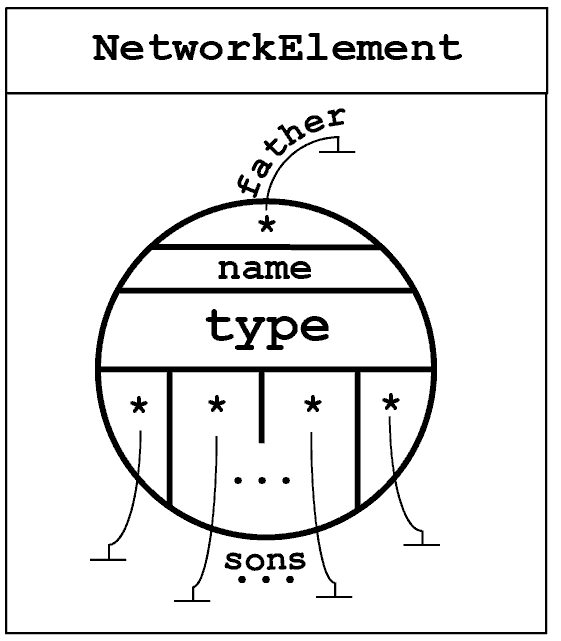
\includegraphics[scale=0.25]{Images/NetworkElement_Object.png}
\end{center}
El diseño de los constructores con y sin argumentos, permite que se pueda instanciar un objeto NetworkElement ya sea asignándole todos los datos necesarios, o bien ninguno. En este último caso, se instancia un Elemento de Red vacío, cuyo esquema es el siguiente:\\
\begin{center}
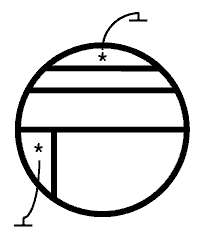
\includegraphics[scale=0.25]{Images/NetworkElement_empty.png}
\end{center}
Luego, los métodos incluídos permiten la asignación de los parámetros del elemento de red, así como la lectura. El código autodocumentado del encabezado de la clase es el detallado en la sección CODE::NetworkElement Class.\\


\subsection{Validación de flujos de entrada y salida}

Para resolver el ingreso y egreso de datos, se utilizó la clase cmdline provista por los docentes.
Esta clase, permite recorrer e identificar las opciones y argumentos con los que se invoca al programa mediante línea de comandos. Luego se definen una serie de métodos que permiten asignar funciones determinadas según las opciones leídas.\\
En particular, se definieron las funciones que deben corresponderse con los argumentos de entrada leídos y validados por cmdline() en archivos denominados \texttt{options.hpp, options.cpp}. Los encabezados de la clase cmdline y de options se aduntan en la sección CODE::cmdline y CODE::options.\\

El tipo de opciones admitidas para este programa están detalladas en los diccionarios globales. El detalle de los diccionarios está en la sección CODE::Dictionary.\\


\subsection{Proceso del archivo de entrada}

Luego de la validación del archivo de entrada, se procede a leer línea po línea el archivo de entrada, ya sea que éste sea un archivo en disco, o bien el flujo de entrada estándar (cin).\\

Se implementó un método de la clase \textit{sstream} que permite operar con un string como si fuera un stream\footnote{método istringstram iss(str)}, y con esto se logró la facilidad de poder identificar las palabras de cada línea mediante el operador sobrecargado $<<$.

\subsubsection{Nombre de Red}

Asumiendo que los archivos de entrada tienen como primera línea el nombre de red, se implementó una función que recibe la cadena de caracteres mediante \textit{getline()} correspondiente a la primer línea del archivo. Esta función desarrollada es \textit{getNetName()} y se encarga de validar que el nombre de red esté bien escrito y lo guarda en un string nomenclado NetName. En caso de que la validación no sea aceptable, se imprime a través del flujo \textit{cerr} el siguiente mensaje de error:\\
\begin{center}
\texttt{error: missing NetworkName}\\
\end{center}

\subsubsection{Vector de Elementos de Red}

Se utilizó la clase Vector de la biblioteca estándar. Por medio de los métodos de inserción, se logró la implementación de un vector dinámico: los elementos de red se validan y se generan de uno en uno, insertandose al final del vector. Con esto se logra que el tamaño del vector quede determinado en tiempo de ejecución. La siguiente imagen representa un esquema de lo que ocurre a medida que el programa lee línea por línea, la clave NetworkElement:\\
\begin{center}
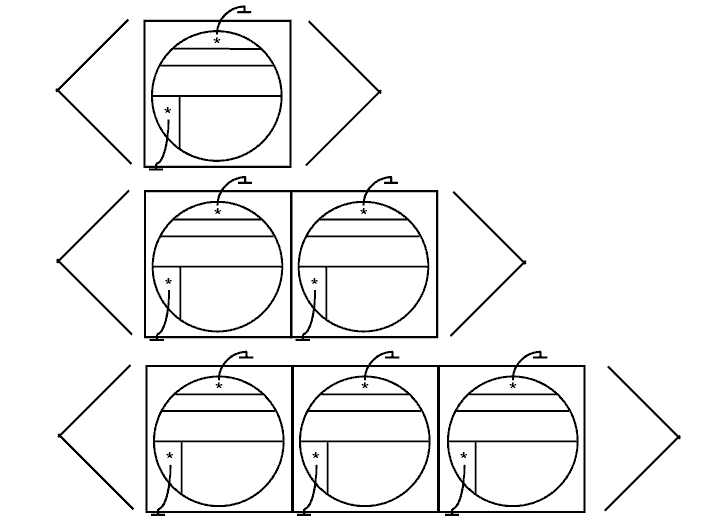
\includegraphics[scale=0.15]{Images/vector_of_NetEls_growing.png}
\end{center}
Básicamente se crea un objeto NetworkElement sin argumentos y se lo adjunta al final del vector, en cada iteración. Una vez finalizada la lectura de NetworkElements, el vector queda completo de objetos y queda determinada la cantidad de elementos de red disponibles en la topología.

\subsubsection{Conexionado}

Para realizar las conexiones correspondientes entre elementos, se procede con la localización y conexión de los elementos que se leen en el texto de entrada bajo el formato: \texttt{Connection <name1> <name2>}. En este punto del programa, ya se dispone del vector de elementos de red completo de objetos con sus respectivos nombres y tipos, por lo que la estrategia pensada resuelve buscar por nombres y conectar los punteros padre y punteros hijo según corresponda.\\

Para lograr esto se implementó un ciclo que recorre el vector desde el primer elemento hasta el último, y que en cada iteración, busca los nombres $<name1>$ y $<name2>$ y los conecta. La figura siguiente es un esquema de lo que realiza el ciclo en este punto del programa:\\
\begin{center}
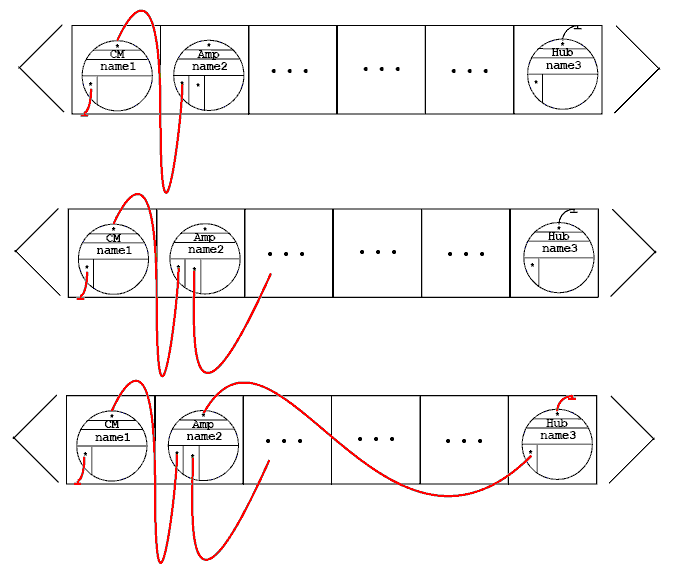
\includegraphics[scale=0.25]{Images/vector_of_NetEls_connecting.png}
\end{center}
Básicamente lee elemento a elemento buscando las claves leídas y conecta los elementos de a uno por vez. El orden no es necesariamente incremental, la imagen es sólo útil para fijar ideas.

\subsection{Detección de loops}

Para la detección de loops, se implementó una función recursiva que básicamente se encarga de recorrer el árbol creado previamente. Recorre en profundidad, saliendo de la misma en caso de detectar ciclos o árboles inconexos. Recibe un entero  por referencia 'vertice' que guarda el numero de conexiones realizadas, y un arreglo de punteros a NetworkElement temporal, donde se guardan la direccion de memoria de los objetos recorridos. La función trabaja de manera recursiva e iterativa garanztizando que siempre que el arbol este armado puede vistar a todos los nodos del mismo.  El valor final que queda guardado en la variable 'vertice' es la cantidad de nodos del arbol excepto la raiz (ver macro ROOT), luego de realizar la funcion "recorrido()".

A partir de este método de recorrido, se implementaron luego pequeñas funciones encargadas de imprimir mensajes de salida si hay elementos repetidos en la topología, si hay ciclos, o bien si hay árboles conexos e inconexos. Las funciones mencionadas son:
\texttt{validateIconnection(); isRepeaten(); validateCycle()}.\\

El detalle de implementación de esta función se puede encontrar en la sección CODE::NetworkElement Class.\\


\subsection{Archivo de salida}

El archivo de salida tiene un formato idéntico al archivo de entrada, pero ahora la información recibida tiene una estructura en memoria. El nombre de red está guardado en la variable NetName. La topología de red está guardada en el vector v, y a partir de recorrer el vector, se imprime el contenido de cada nodo en el siguiente formato: \\
\texttt{NetworkElement <name> <type>}\\
Luego se recorre nuevamente el vector y se imprimen las conexiones en el siguiente formato:\\
\texttt{Connection <sons> <name> }\\
Esta última línea merece una explicación, pues la impresión de \texttt{<sons>} se realiza de forma iterativa para todos los elementos de red hijos que tiene el nodo posicionado de nombre \texttt{<name>}.\\

\section{Ejecuciones}

\subsection{Compilación}
La compilación del programa se realiza por medio de un Makefile. El detalle se encuentra en la sección CODE::Makefile. Como salida, se genera un archivo ejecutable de extension.exe.

Para ejecutar el programa se necesita invocar con la siguiente línea de comandos:
\texttt{$./main_TP1.exe -i <entrada.txt> -o <salida.txt>$}
Las pruebas que se realizaron contemplan archivos correctos de entrada, y algunos ejemplos que contienen topologías inconexas y topologías con ciclos. Los resultados se adjuntan a continuación:\\
\title{Entrada correcta}\\
\begin{center}
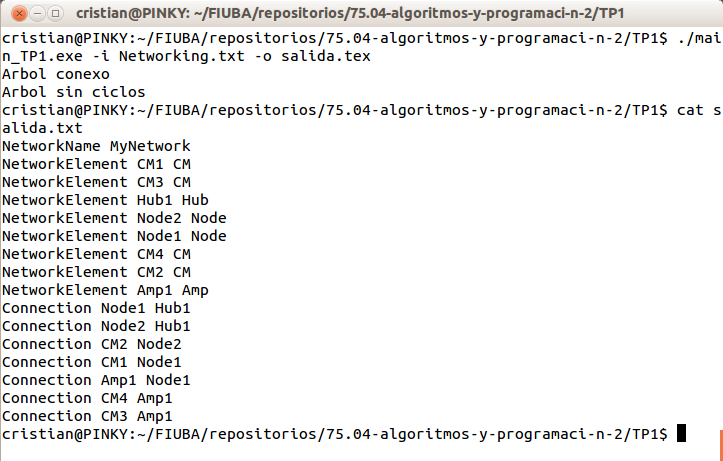
\includegraphics[scale=0.25]{Images/test1.png}\\
\end{center}\title{Entrada de malas conexiones}\\
\title{Entrada de árbol inconexo}\\
\begin{center}
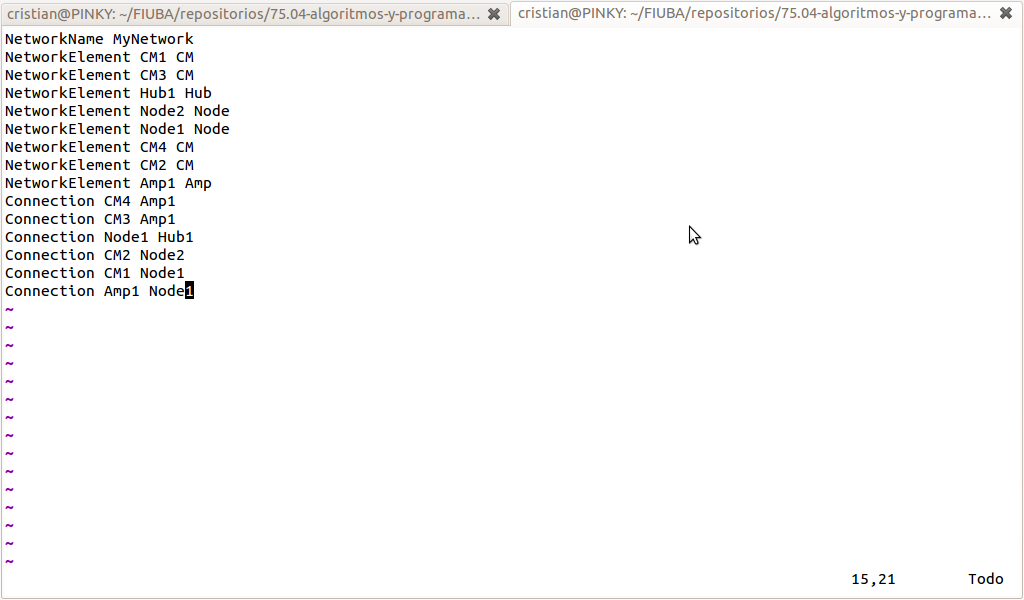
\includegraphics[scale=0.25]{Images/entrada de arbol inconexo.png}\\
\end{center}\title{Entrada de malas conexiones}\\
\begin{center}
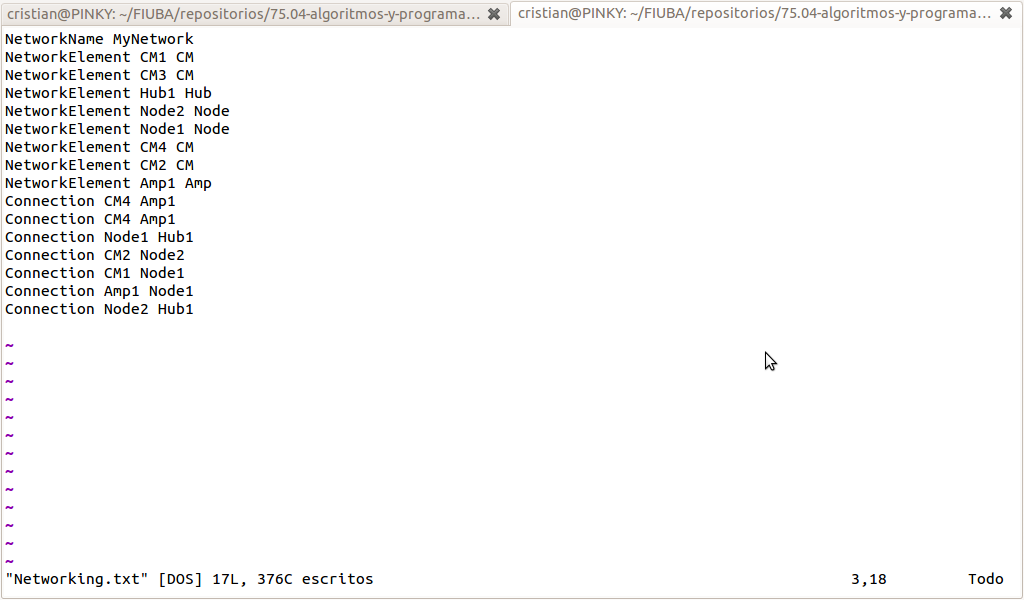
\includegraphics[scale=0.25]{Images/entrada de malas conexiones.png}\\
\end{center}\title{Entrada de múltiple nodos}\\
\begin{center}
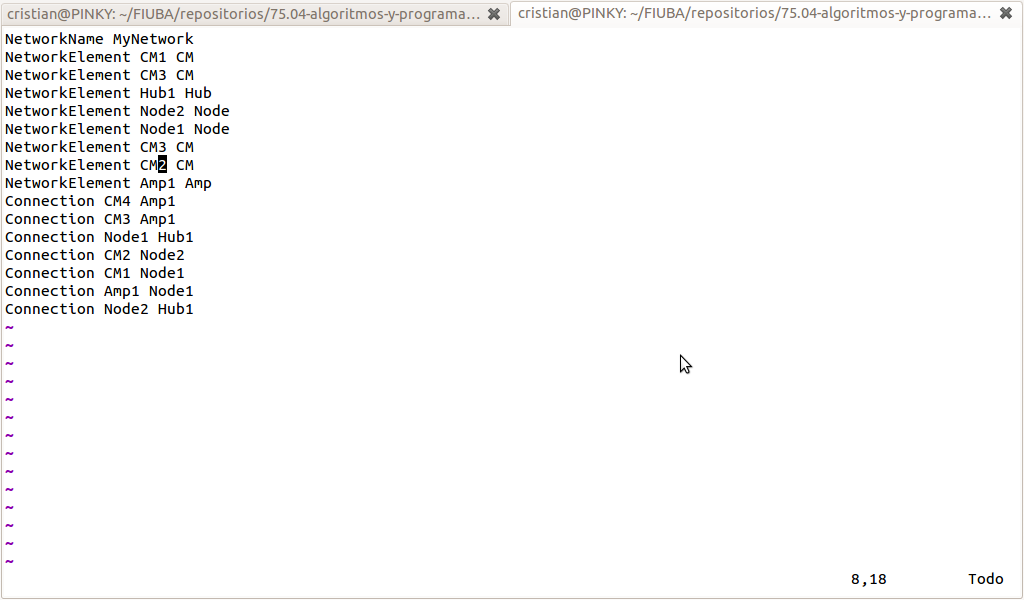
\includegraphics[scale=0.25]{Images/entrada de multiple nodos.png}\\
\end{center}\title{Malas conexiones}\\
\begin{center}
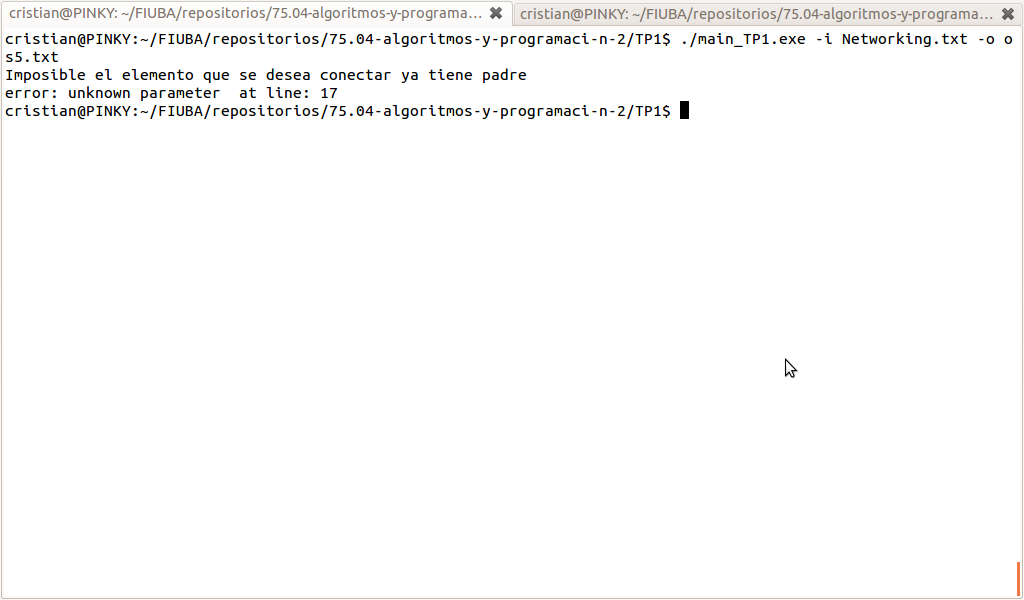
\includegraphics[scale=0.25]{Images/malas conexiones.png}\\
\end{center}\title{Múltiple nodos}\\
\begin{center}
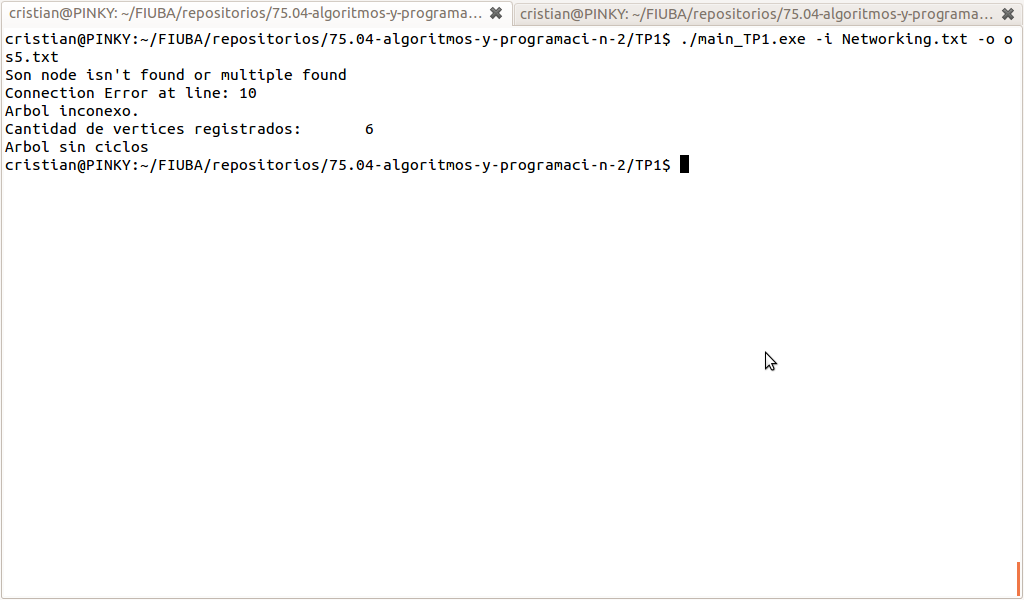
\includegraphics[scale=0.25]{Images/multiple nodos.png}\\
\end{center}
\subsection{Comprobación de uso de memoria con Valgrind}
Utilizando la ejecucion del programa Valgrind bajo el siguiente formato:\\
\texttt{$valgrind --tool=memcheck ./main_TP1.exe -i Networking.txt -o salida.txt$}\\
se obtiene el siguiente resultado:\\
\begin{center}
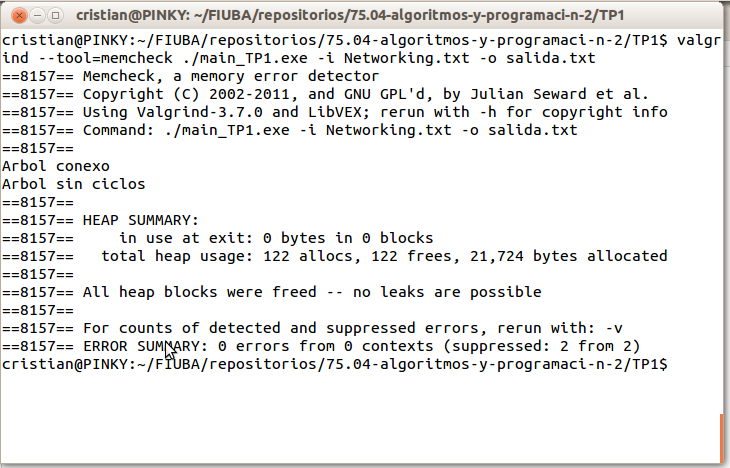
\includegraphics[scale=0.25]{Images/vagrind2.png}\\
\end{center}que verifica que no hay fugas de memoria.

\section{Códigos}
%Los códigos no deben tener \textbf{\underline{texto acentuado}}.
\subsection*{CODE::Makefile}
\lstinputlisting{Codes/makefile}

\subsection*{CODE::main}
\lstinputlisting{Codes/main_TP1.cpp}

\subsection*{CODE::Dictionary}
\lstinputlisting{Codes/dictionary.hpp}
\lstinputlisting{Codes/dictionary.cpp}

\subsection*{CODE::NetworkElement Class}
\lstinputlisting{Codes/NetworkElementClass.hpp}
\lstinputlisting{Codes/NetworkElementClass.cpp}

\subsection*{CODE::cmdline}
\lstinputlisting{Codes/cmdline.h}
\lstinputlisting{Codes/cmdline.cc}

\subsection*{CODE::option}
\lstinputlisting{Codes/options.hpp}
\lstinputlisting{Codes/options.cpp}

\subsection*{CODE::process}
\lstinputlisting{Codes/process.hpp}
\lstinputlisting{Codes/process.cpp}

\end{document}